\documentclass[tikz,border=8pt]{standalone}
% Shared look for every TikZ diagram. Load with \input{../../tools/tikz-style.tex}
\usepackage[T1]{fontenc}
\usepackage{lmodern}
\renewcommand{\sfdefault}{lmr}  % diagrams use the same serif as the text
\usetikzlibrary{arrows.meta, positioning, shapes.geometric, calc, fit, backgrounds}
\definecolor{cblue}{HTML}{4C78A8}
\definecolor{corange}{HTML}{F58518}
\definecolor{cgreen}{HTML}{54A24B}
\definecolor{cred}{HTML}{E45756}
\definecolor{cpurple}{HTML}{B279A2}
\definecolor{cgrey}{HTML}{6B6B6B}
\tikzset{
  every picture/.style={font=\sffamily, line width=1.2pt},
  box/.style={draw=#1, fill=#1!12, rounded corners=4pt, align=center, inner sep=7pt, minimum height=1.1cm},
  box/.default=cgrey,
  arrow/.style={-{Stealth[length=3mm]}, draw=cgrey, line width=1.4pt},
  title/.style={font=\sffamily\bfseries\Large},
  note/.style={font=\sffamily\small, text=cgrey, align=center},
}
\AtBeginDocument{\hyphenpenalty=10000 \exhyphenpenalty=10000}

\begin{document}
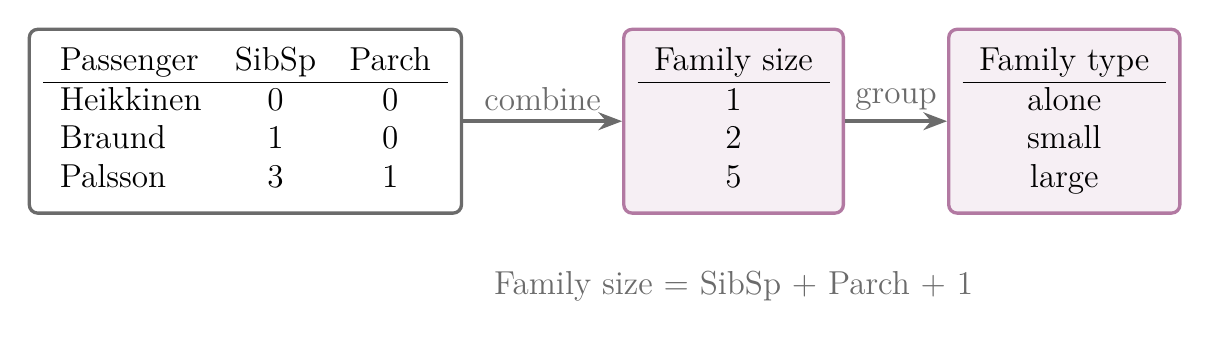
\begin{tikzpicture}[every node/.append style={font=\sffamily\large}]
\tikzset{note/.style={font=\sffamily\large, text=cgrey, align=center}}
  \tikzset{tab/.style={draw=cgrey, fill=white, rounded corners=3pt, inner sep=5pt, font=\sffamily\large}}
  \node[tab] (a) at (0,0) {\begin{tabular}{lcc}Passenger & SibSp & Parch\\\hline Heikkinen & 0 & 0\\Braund & 1 & 0\\Palsson & 3 & 1\end{tabular}};
  \node[tab, draw=cpurple, fill=cpurple!12] (b) at (6.2,0) {\begin{tabular}{c}Family size\\\hline 1\\2\\5\end{tabular}};
  \node[tab, draw=cpurple, fill=cpurple!12] (c) at (10.4,0) {\begin{tabular}{c}Family type\\\hline alone\\small\\large\end{tabular}};
  \draw[arrow] (a) -- node[above, note] {combine} (b);
  \draw[arrow] (b) -- node[above, note] {group} (c);
  \node[note] at (6.2,-2.1) {Family size = SibSp + Parch + 1};
\end{tikzpicture}
\end{document}
